% Options for packages loaded elsewhere
\PassOptionsToPackage{unicode}{hyperref}
\PassOptionsToPackage{hyphens}{url}
%
\documentclass[
]{article}
\usepackage{amsmath,amssymb}
\usepackage{lmodern}
\usepackage{iftex}
\ifPDFTeX
  \usepackage[T1]{fontenc}
  \usepackage[utf8]{inputenc}
  \usepackage{textcomp} % provide euro and other symbols
\else % if luatex or xetex
  \usepackage{unicode-math}
  \defaultfontfeatures{Scale=MatchLowercase}
  \defaultfontfeatures[\rmfamily]{Ligatures=TeX,Scale=1}
\fi
% Use upquote if available, for straight quotes in verbatim environments
\IfFileExists{upquote.sty}{\usepackage{upquote}}{}
\IfFileExists{microtype.sty}{% use microtype if available
  \usepackage[]{microtype}
  \UseMicrotypeSet[protrusion]{basicmath} % disable protrusion for tt fonts
}{}
\makeatletter
\@ifundefined{KOMAClassName}{% if non-KOMA class
  \IfFileExists{parskip.sty}{%
    \usepackage{parskip}
  }{% else
    \setlength{\parindent}{0pt}
    \setlength{\parskip}{6pt plus 2pt minus 1pt}}
}{% if KOMA class
  \KOMAoptions{parskip=half}}
\makeatother
\usepackage{xcolor}
\usepackage[margin=1in]{geometry}
\usepackage{color}
\usepackage{fancyvrb}
\newcommand{\VerbBar}{|}
\newcommand{\VERB}{\Verb[commandchars=\\\{\}]}
\DefineVerbatimEnvironment{Highlighting}{Verbatim}{commandchars=\\\{\}}
% Add ',fontsize=\small' for more characters per line
\usepackage{framed}
\definecolor{shadecolor}{RGB}{248,248,248}
\newenvironment{Shaded}{\begin{snugshade}}{\end{snugshade}}
\newcommand{\AlertTok}[1]{\textcolor[rgb]{0.94,0.16,0.16}{#1}}
\newcommand{\AnnotationTok}[1]{\textcolor[rgb]{0.56,0.35,0.01}{\textbf{\textit{#1}}}}
\newcommand{\AttributeTok}[1]{\textcolor[rgb]{0.77,0.63,0.00}{#1}}
\newcommand{\BaseNTok}[1]{\textcolor[rgb]{0.00,0.00,0.81}{#1}}
\newcommand{\BuiltInTok}[1]{#1}
\newcommand{\CharTok}[1]{\textcolor[rgb]{0.31,0.60,0.02}{#1}}
\newcommand{\CommentTok}[1]{\textcolor[rgb]{0.56,0.35,0.01}{\textit{#1}}}
\newcommand{\CommentVarTok}[1]{\textcolor[rgb]{0.56,0.35,0.01}{\textbf{\textit{#1}}}}
\newcommand{\ConstantTok}[1]{\textcolor[rgb]{0.00,0.00,0.00}{#1}}
\newcommand{\ControlFlowTok}[1]{\textcolor[rgb]{0.13,0.29,0.53}{\textbf{#1}}}
\newcommand{\DataTypeTok}[1]{\textcolor[rgb]{0.13,0.29,0.53}{#1}}
\newcommand{\DecValTok}[1]{\textcolor[rgb]{0.00,0.00,0.81}{#1}}
\newcommand{\DocumentationTok}[1]{\textcolor[rgb]{0.56,0.35,0.01}{\textbf{\textit{#1}}}}
\newcommand{\ErrorTok}[1]{\textcolor[rgb]{0.64,0.00,0.00}{\textbf{#1}}}
\newcommand{\ExtensionTok}[1]{#1}
\newcommand{\FloatTok}[1]{\textcolor[rgb]{0.00,0.00,0.81}{#1}}
\newcommand{\FunctionTok}[1]{\textcolor[rgb]{0.00,0.00,0.00}{#1}}
\newcommand{\ImportTok}[1]{#1}
\newcommand{\InformationTok}[1]{\textcolor[rgb]{0.56,0.35,0.01}{\textbf{\textit{#1}}}}
\newcommand{\KeywordTok}[1]{\textcolor[rgb]{0.13,0.29,0.53}{\textbf{#1}}}
\newcommand{\NormalTok}[1]{#1}
\newcommand{\OperatorTok}[1]{\textcolor[rgb]{0.81,0.36,0.00}{\textbf{#1}}}
\newcommand{\OtherTok}[1]{\textcolor[rgb]{0.56,0.35,0.01}{#1}}
\newcommand{\PreprocessorTok}[1]{\textcolor[rgb]{0.56,0.35,0.01}{\textit{#1}}}
\newcommand{\RegionMarkerTok}[1]{#1}
\newcommand{\SpecialCharTok}[1]{\textcolor[rgb]{0.00,0.00,0.00}{#1}}
\newcommand{\SpecialStringTok}[1]{\textcolor[rgb]{0.31,0.60,0.02}{#1}}
\newcommand{\StringTok}[1]{\textcolor[rgb]{0.31,0.60,0.02}{#1}}
\newcommand{\VariableTok}[1]{\textcolor[rgb]{0.00,0.00,0.00}{#1}}
\newcommand{\VerbatimStringTok}[1]{\textcolor[rgb]{0.31,0.60,0.02}{#1}}
\newcommand{\WarningTok}[1]{\textcolor[rgb]{0.56,0.35,0.01}{\textbf{\textit{#1}}}}
\usepackage{graphicx}
\makeatletter
\def\maxwidth{\ifdim\Gin@nat@width>\linewidth\linewidth\else\Gin@nat@width\fi}
\def\maxheight{\ifdim\Gin@nat@height>\textheight\textheight\else\Gin@nat@height\fi}
\makeatother
% Scale images if necessary, so that they will not overflow the page
% margins by default, and it is still possible to overwrite the defaults
% using explicit options in \includegraphics[width, height, ...]{}
\setkeys{Gin}{width=\maxwidth,height=\maxheight,keepaspectratio}
% Set default figure placement to htbp
\makeatletter
\def\fps@figure{htbp}
\makeatother
\setlength{\emergencystretch}{3em} % prevent overfull lines
\providecommand{\tightlist}{%
  \setlength{\itemsep}{0pt}\setlength{\parskip}{0pt}}
\setcounter{secnumdepth}{-\maxdimen} % remove section numbering
\ifLuaTeX
  \usepackage{selnolig}  % disable illegal ligatures
\fi
\IfFileExists{bookmark.sty}{\usepackage{bookmark}}{\usepackage{hyperref}}
\IfFileExists{xurl.sty}{\usepackage{xurl}}{} % add URL line breaks if available
\urlstyle{same} % disable monospaced font for URLs
\hypersetup{
  pdftitle={Testing Figure 1},
  hidelinks,
  pdfcreator={LaTeX via pandoc}}

\title{Testing Figure 1}
\author{}
\date{\vspace{-2.5em}2022-11-18}

\begin{document}
\maketitle

\begin{quote}
Working on our initial report, it became evident that the raw data from
Cavanna et al.~(2021), ``Lifetime use of psychedelics is associated with
better mental health indicators during the COVID-19 pandemic'' would not
be appropriate to use for all aspects of the Final Project for PSYC
201A. The authors of said paper applied some exclusion criteria to their
data which we simply would not be able to replicate, and this became
apparent as we first attempted to replicate their exclusion criteria and
then to replicate some of their statistical findings. Faced with a
difficult decision, we opted to replicate the results and perform novel
analysis on a similar paper: ``Psychedelic mushrooms in the USA:
Knowledge, patterns of use, and association with health outcomes,'' by
Matzopoulos, Morlock, Morlock, Lerer \& Lerer (2021). In this open
dataset, we continued to find publication decisions on the part of
authors which complicate complete replication, but feel they have
provided sufficient data to allow for partial replication of some
published results and novel analysis. We reviewed about ten papers in
our search for a dataset for this project and learned a valuable lesson.
We believe the challenges we've faced in finding an appropriate open
dataset potentially reflect facets of an ongoing replication crisis in
the fields of shared interest to us and highlight the importance of
rigorous and open science as we move forward in our careers.
\end{quote}

\begin{quote}
Matzopoulos, Morlock, Morlock, Lerer \& Lerer (2021) examined the use of
psychedelic mushrooms (PM) in association with measures of mental health
status and outcomes and quality of life. They examined participants'
motivations for consumption of PM including desires for general mental
health and well-being, as medication for medically diagnosed conditions,
and as self-medication for undiagnosed conditions. The authors observed
that users of PM reported more depression and anxiety as measured by the
GAD-7 and PHQ-9, as well as several other factors predictive of PM use
such as gender and not having health insurance. Examining a sample of
7,139 participants weighted to current estimates of the US population,
the authors report that a significant number of US adults are already
self-medicating with PM. Positive press coverage and ``hype'' indicate
that this proportion of the population is likely to increase, and this
necessitates further research into the association between PM use and
poor mental health outcomes.
\end{quote}

\hypertarget{link-to-paper-and-dataset}{%
\subsection{Link to paper and
dataset:}\label{link-to-paper-and-dataset}}

\hypertarget{published-paper-permalink-httpswww.ncbi.nlm.nih.govpmcarticlespmc8761614}{%
\subsection{\texorpdfstring{Published paper permalink:
\url{https://www.ncbi.nlm.nih.gov/pmc/articles/PMC8761614/}}{Published paper permalink: https://www.ncbi.nlm.nih.gov/pmc/articles/PMC8761614/}}\label{published-paper-permalink-httpswww.ncbi.nlm.nih.govpmcarticlespmc8761614}}

\hypertarget{dataset-available-via-zenodo-httpszenodo.orgrecord5791226.y3lgfuzmkro}{%
\subsection{\texorpdfstring{Dataset available via Zenodo:
\url{https://zenodo.org/record/5791226\#.Y3lGFuzMKrO}}{Dataset available via Zenodo: https://zenodo.org/record/5791226\#.Y3lGFuzMKrO}}\label{dataset-available-via-zenodo-httpszenodo.orgrecord5791226.y3lgfuzmkro}}

\begin{Shaded}
\begin{Highlighting}[]
\FunctionTok{library}\NormalTok{(tidyverse)}
\end{Highlighting}
\end{Shaded}

\begin{verbatim}
## -- Attaching packages --------------------------------------- tidyverse 1.3.2 --
## v ggplot2 3.3.6      v purrr   0.3.4 
## v tibble  3.1.8      v dplyr   1.0.10
## v tidyr   1.2.1      v stringr 1.4.1 
## v readr   2.1.2      v forcats 0.5.2 
## -- Conflicts ------------------------------------------ tidyverse_conflicts() --
## x dplyr::filter() masks stats::filter()
## x dplyr::lag()    masks stats::lag()
\end{verbatim}

\hypertarget{replication-of-figure-1-figure-1-represents-a-multivariate-logistic-regression-model-using-predictive-factors-to-predict-use-of-pm.-predictive-factors-of-pm-use-include-being-male-having-a-higher-score-on-the-charlson-comorbidity-index-or-living-in-the-western-census-region-of-the-us.-self-report-of-pm-use-was-less-likely-among-participants-who-had-health-insurance-were-relatively-older-or-who-lived-outside-of-the-western-us-census-region-i.e.-in-the-northeast-midwest-or-south.-these-relationships-are-reported-as-odds-ratios-ors-and-95-confidence-intervals-95-ci-lower-upper.}{%
\subsection{Replication of Figure 1: Figure 1 represents a multivariate
logistic regression model using predictive factors to predict use of PM.
Predictive factors of PM use include being male, having a higher score
on the Charlson Comorbidity Index, or living in the Western Census
Region of the US. Self-report of PM use was less likely among
participants who had health insurance, were relatively older, or who
lived outside of the Western US Census region (i.e., in the Northeast,
Midwest, or South). These relationships are reported as odds ratios
(ORs) and 95\% Confidence Intervals (95\% CI; lower,
upper).}\label{replication-of-figure-1-figure-1-represents-a-multivariate-logistic-regression-model-using-predictive-factors-to-predict-use-of-pm.-predictive-factors-of-pm-use-include-being-male-having-a-higher-score-on-the-charlson-comorbidity-index-or-living-in-the-western-census-region-of-the-us.-self-report-of-pm-use-was-less-likely-among-participants-who-had-health-insurance-were-relatively-older-or-who-lived-outside-of-the-western-us-census-region-i.e.-in-the-northeast-midwest-or-south.-these-relationships-are-reported-as-odds-ratios-ors-and-95-confidence-intervals-95-ci-lower-upper.}}

\hypertarget{load-data}{%
\subsection{Load data}\label{load-data}}

\begin{Shaded}
\begin{Highlighting}[]
\NormalTok{PM }\OtherTok{=} \FunctionTok{read.csv}\NormalTok{(}\StringTok{\textquotesingle{}data/external/AHRI\_DATASET\_PM\_MANUSCRIPT\_DATA.csv\textquotesingle{}}\NormalTok{)}
\end{Highlighting}
\end{Shaded}

\hypertarget{clean-data}{%
\subsection{Clean data}\label{clean-data}}

\begin{Shaded}
\begin{Highlighting}[]
\CommentTok{\# only necessary columns for figure 1\textquotesingle{}s multivariate logistical regression}
\NormalTok{PM\_cleaned }\OtherTok{=}\NormalTok{ PM }\SpecialCharTok{\%\textgreater{}\%}
  \FunctionTok{select}\NormalTok{(}
\NormalTok{    CASEID\_7139, }
\NormalTok{    SEX, }
\NormalTok{    AGE, }
\NormalTok{    ETHNICITY, }
\NormalTok{    HLS\_YN,}
\NormalTok{    REGION, }
\NormalTok{    CCI\_SCORE, }
\NormalTok{    GAD7\_GE10, }
\NormalTok{    PHQ9\_GE10, }
\NormalTok{    INSURANCE, }
\NormalTok{    PM1\_GEN\_HEALTH, }
\NormalTok{    PM1\_DIAG\_CONDITION, }
\NormalTok{    PM1\_UNDIAG\_CONCERN}
\NormalTok{    ) }\SpecialCharTok{\%\textgreater{}\%}
  \FunctionTok{mutate}\NormalTok{(}
    \AttributeTok{PM\_12M =}\NormalTok{ PM1\_GEN\_HEALTH }\SpecialCharTok{+}\NormalTok{ PM1\_UNDIAG\_CONCERN }\SpecialCharTok{+}\NormalTok{ PM1\_DIAG\_CONDITION}
\NormalTok{    )}

\CommentTok{\# calculate boolean for PM\_12M}
\NormalTok{PM\_cleaned}\SpecialCharTok{$}\NormalTok{PM\_12M }\OtherTok{=}\NormalTok{ PM\_cleaned}\SpecialCharTok{$}\NormalTok{PM\_12M }\SpecialCharTok{\%\textgreater{}\%}
  \FunctionTok{recode}\NormalTok{(}\StringTok{\textasciigrave{}}\AttributeTok{{-}297}\StringTok{\textasciigrave{}} \OtherTok{=} \DecValTok{0}\NormalTok{, }\StringTok{\textasciigrave{}}\AttributeTok{0}\StringTok{\textasciigrave{}} \OtherTok{=} \DecValTok{0}\NormalTok{, }\StringTok{\textasciigrave{}}\AttributeTok{1}\StringTok{\textasciigrave{}} \OtherTok{=} \DecValTok{1}\NormalTok{, }\StringTok{\textasciigrave{}}\AttributeTok{2}\StringTok{\textasciigrave{}} \OtherTok{=} \DecValTok{1}\NormalTok{, }\StringTok{\textasciigrave{}}\AttributeTok{3}\StringTok{\textasciigrave{}} \OtherTok{=} \DecValTok{1}\NormalTok{)}
\end{Highlighting}
\end{Shaded}

\begin{Shaded}
\begin{Highlighting}[]
\DocumentationTok{\#\# refactor columns}
\NormalTok{PM\_cleaned}\SpecialCharTok{$}\NormalTok{SEX }\OtherTok{=}\NormalTok{ PM\_cleaned}\SpecialCharTok{$}\NormalTok{SEX }\SpecialCharTok{\%\textgreater{}\%}
  \FunctionTok{recode\_factor}\NormalTok{(., }\StringTok{\textasciigrave{}}\AttributeTok{0}\StringTok{\textasciigrave{}} \OtherTok{=} \StringTok{\textquotesingle{}Female\textquotesingle{}}\NormalTok{, }\StringTok{\textasciigrave{}}\AttributeTok{1}\StringTok{\textasciigrave{}} \OtherTok{=} \StringTok{\textquotesingle{}Male\textquotesingle{}}\NormalTok{)}

\NormalTok{PM\_cleaned}\SpecialCharTok{$}\NormalTok{ETHNICITY }\OtherTok{=}\NormalTok{ PM\_cleaned}\SpecialCharTok{$}\NormalTok{ETHNICITY }\SpecialCharTok{\%\textgreater{}\%}
  \FunctionTok{recode\_factor}\NormalTok{(., }\StringTok{\textasciigrave{}}\AttributeTok{1}\StringTok{\textasciigrave{}} \OtherTok{=} \StringTok{\textquotesingle{}Other\textquotesingle{}}\NormalTok{, }\StringTok{\textasciigrave{}}\AttributeTok{2}\StringTok{\textasciigrave{}} \OtherTok{=} \StringTok{\textquotesingle{}White\textquotesingle{}}\NormalTok{, }\StringTok{\textasciigrave{}}\AttributeTok{3}\StringTok{\textasciigrave{}} \OtherTok{=} \StringTok{\textquotesingle{}Other\textquotesingle{}}\NormalTok{)}

\NormalTok{PM\_cleaned}\SpecialCharTok{$}\NormalTok{HLS\_YN }\OtherTok{=}\NormalTok{ PM\_cleaned}\SpecialCharTok{$}\NormalTok{HLS\_YN }\SpecialCharTok{\%\textgreater{}\%}
  \FunctionTok{recode\_factor}\NormalTok{(., }\StringTok{\textasciigrave{}}\AttributeTok{0}\StringTok{\textasciigrave{}} \OtherTok{=} \StringTok{\textquotesingle{}None{-}Hispanic\textquotesingle{}}\NormalTok{, }\StringTok{\textasciigrave{}}\AttributeTok{1}\StringTok{\textasciigrave{}} \OtherTok{=} \StringTok{\textquotesingle{}Hispanic\textquotesingle{}}\NormalTok{)}

\NormalTok{PM\_cleaned}\SpecialCharTok{$}\NormalTok{REGION }\OtherTok{=}\NormalTok{ PM\_cleaned}\SpecialCharTok{$}\NormalTok{REGION }\SpecialCharTok{\%\textgreater{}\%}
  \FunctionTok{recode\_factor}\NormalTok{(.,}\StringTok{\textasciigrave{}}\AttributeTok{1}\StringTok{\textasciigrave{}} \OtherTok{=} \StringTok{\textquotesingle{}Northeast\textquotesingle{}}\NormalTok{, }\StringTok{\textasciigrave{}}\AttributeTok{2}\StringTok{\textasciigrave{}} \OtherTok{=} \StringTok{\textquotesingle{}Midwest\textquotesingle{}}\NormalTok{, }\StringTok{\textasciigrave{}}\AttributeTok{3}\StringTok{\textasciigrave{}} \OtherTok{=} \StringTok{\textquotesingle{}South\textquotesingle{}}\NormalTok{, }\StringTok{\textasciigrave{}}\AttributeTok{4}\StringTok{\textasciigrave{}} \OtherTok{=} \StringTok{\textquotesingle{}West\textquotesingle{}}\NormalTok{)}
\end{Highlighting}
\end{Shaded}

\hypertarget{multivariate-logistical-regression}{%
\subsection{Multivariate logistical
regression}\label{multivariate-logistical-regression}}

\begin{Shaded}
\begin{Highlighting}[]
\DocumentationTok{\#\# modified helper from https://rdrr.io/github/eringrand/RUncommon/src/R/logistic.regression.or.ci.R}
\NormalTok{logistic.regression.or.ci }\OtherTok{\textless{}{-}} \ControlFlowTok{function}\NormalTok{(regress.out, }\AttributeTok{level =} \FloatTok{0.95}\NormalTok{) \{}
\NormalTok{  usual.output }\OtherTok{\textless{}{-}} \FunctionTok{summary}\NormalTok{(regress.out)}
\NormalTok{  z.quantile }\OtherTok{\textless{}{-}}\NormalTok{ stats}\SpecialCharTok{::}\FunctionTok{qnorm}\NormalTok{(}\DecValTok{1} \SpecialCharTok{{-}}\NormalTok{ (}\DecValTok{1} \SpecialCharTok{{-}}\NormalTok{ level) }\SpecialCharTok{/} \DecValTok{2}\NormalTok{)}
\NormalTok{  number.vars }\OtherTok{\textless{}{-}} \FunctionTok{length}\NormalTok{(regress.out}\SpecialCharTok{$}\NormalTok{coefficients)}
\NormalTok{  OR }\OtherTok{\textless{}{-}} \FunctionTok{exp}\NormalTok{(regress.out}\SpecialCharTok{$}\NormalTok{coefficients[}\SpecialCharTok{{-}}\DecValTok{1}\NormalTok{])}
\NormalTok{  temp.store.result }\OtherTok{\textless{}{-}} \FunctionTok{matrix}\NormalTok{(}\FunctionTok{rep}\NormalTok{(}\ConstantTok{NA}\NormalTok{, number.vars }\SpecialCharTok{*} \DecValTok{2}\NormalTok{), }\AttributeTok{nrow =}\NormalTok{ number.vars)}
  \ControlFlowTok{for}\NormalTok{ (i }\ControlFlowTok{in} \DecValTok{1}\SpecialCharTok{:}\NormalTok{number.vars) \{}
\NormalTok{    temp.store.result[i, ] }\OtherTok{\textless{}{-}} \FunctionTok{summary}\NormalTok{(regress.out)}\SpecialCharTok{$}\NormalTok{coefficients[i] }\SpecialCharTok{+}
      \FunctionTok{c}\NormalTok{(}\SpecialCharTok{{-}}\DecValTok{1}\NormalTok{, }\DecValTok{1}\NormalTok{) }\SpecialCharTok{*}\NormalTok{ z.quantile }\SpecialCharTok{*} \FunctionTok{summary}\NormalTok{(regress.out)}\SpecialCharTok{$}\NormalTok{coefficients[i }\SpecialCharTok{+}\NormalTok{ number.vars]}
\NormalTok{  \}}
\NormalTok{  intercept.ci }\OtherTok{\textless{}{-}}\NormalTok{ temp.store.result[}\DecValTok{1}\NormalTok{, ]}
\NormalTok{  slopes.ci }\OtherTok{\textless{}{-}}\NormalTok{ temp.store.result[}\SpecialCharTok{{-}}\DecValTok{1}\NormalTok{, ]}
\NormalTok{  OR.ci }\OtherTok{\textless{}{-}} \FunctionTok{exp}\NormalTok{(slopes.ci)}
  
\NormalTok{  output }\OtherTok{\textless{}{-}} \FunctionTok{list}\NormalTok{(}
    \AttributeTok{regression.table =}\NormalTok{ usual.output, }\AttributeTok{intercept.ci =}\NormalTok{ intercept.ci,}
    \AttributeTok{slopes.ci =}\NormalTok{ slopes.ci, }\AttributeTok{OR =}\NormalTok{ OR, }\AttributeTok{OR.ci =}\NormalTok{ OR.ci}
\NormalTok{  )}
  \FunctionTok{return}\NormalTok{(output)}
\NormalTok{\}}
\end{Highlighting}
\end{Shaded}

\begin{Shaded}
\begin{Highlighting}[]
\NormalTok{full\_model }\OtherTok{=} \FunctionTok{glm}\NormalTok{(PM\_12M }\SpecialCharTok{\textasciitilde{}}\NormalTok{ SEX }\SpecialCharTok{+}\NormalTok{ AGE }\SpecialCharTok{+}\NormalTok{ ETHNICITY }\SpecialCharTok{+}\NormalTok{ REGION }\SpecialCharTok{+}\NormalTok{ CCI\_SCORE }\SpecialCharTok{+}\NormalTok{ GAD7\_GE10 }\SpecialCharTok{+}\NormalTok{ PHQ9\_GE10 }\SpecialCharTok{+}\NormalTok{ INSURANCE, }\AttributeTok{data =}\NormalTok{ PM\_cleaned, }\AttributeTok{family =}\NormalTok{ binomial)}
\NormalTok{full\_model\_results }\OtherTok{=} \FunctionTok{logistic.regression.or.ci}\NormalTok{(full\_model)}
\NormalTok{full\_model\_results}
\end{Highlighting}
\end{Shaded}

\begin{verbatim}
## $regression.table
## 
## Call:
## glm(formula = PM_12M ~ SEX + AGE + ETHNICITY + REGION + CCI_SCORE + 
##     GAD7_GE10 + PHQ9_GE10 + INSURANCE, family = binomial, data = PM_cleaned)
## 
## Deviance Residuals: 
##     Min       1Q   Median       3Q      Max  
## -0.9536  -0.2812  -0.1814  -0.1113   3.3346  
## 
## Coefficients:
##                 Estimate Std. Error z value Pr(>|z|)    
## (Intercept)    -3.182061   0.361780  -8.796  < 2e-16 ***
## SEXMale         1.002818   0.148650   6.746 1.52e-11 ***
## AGE            -0.048536   0.006197  -7.832 4.79e-15 ***
## ETHNICITYWhite  0.493329   0.168726   2.924  0.00346 ** 
## REGIONMidwest  -0.082923   0.245897  -0.337  0.73595    
## REGIONSouth     0.144182   0.211860   0.681  0.49616    
## REGIONWest      0.388157   0.221003   1.756  0.07903 .  
## CCI_SCORE       0.247087   0.058807   4.202 2.65e-05 ***
## GAD7_GE10       0.247902   0.177679   1.395  0.16295    
## PHQ9_GE10       0.976374   0.186931   5.223 1.76e-07 ***
## INSURANCE      -0.067125   0.170770  -0.393  0.69427    
## ---
## Signif. codes:  0 '***' 0.001 '**' 0.01 '*' 0.05 '.' 0.1 ' ' 1
## 
## (Dispersion parameter for binomial family taken to be 1)
## 
##     Null deviance: 2019.1  on 7138  degrees of freedom
## Residual deviance: 1766.5  on 7128  degrees of freedom
## AIC: 1788.5
## 
## Number of Fisher Scoring iterations: 7
## 
## 
## $intercept.ci
## [1] -3.891137 -2.472984
## 
## $slopes.ci
##              [,1]        [,2]
##  [1,]  0.71146923  1.29416691
##  [2,] -0.06068113 -0.03638991
##  [3,]  0.16263260  0.82402449
##  [4,] -0.56487200  0.39902653
##  [5,] -0.27105703  0.55942005
##  [6,] -0.04500019  0.82131482
##  [7,]  0.13182829  0.36234554
##  [8,] -0.10034179  0.59614668
##  [9,]  0.60999473  1.34275255
## [10,] -0.40182830  0.26757920
## 
## $OR
##        SEXMale            AGE ETHNICITYWhite  REGIONMidwest    REGIONSouth 
##      2.7259529      0.9526235      1.6377585      0.9204223      1.1550938 
##     REGIONWest      CCI_SCORE      GAD7_GE10      PHQ9_GE10      INSURANCE 
##      1.4742617      1.2802904      1.2813349      2.6548115      0.9350787 
## 
## $OR.ci
##            [,1]      [,2]
##  [1,] 2.0369818 3.6479556
##  [2,] 0.9411233 0.9642642
##  [3,] 1.1766043 2.2796559
##  [4,] 0.5684329 1.4903732
##  [5,] 0.7625730 1.7496575
##  [6,] 0.9559973 2.2734871
##  [7,] 1.1409124 1.4366953
##  [8,] 0.9045282 1.8151111
##  [9,] 1.8404217 3.8295701
## [10,] 0.6690956 1.3067971
\end{verbatim}

\begin{Shaded}
\begin{Highlighting}[]
\NormalTok{figure1df }\OtherTok{=} \FunctionTok{data.frame}\NormalTok{(full\_model\_results}\SpecialCharTok{$}\NormalTok{OR)}
\NormalTok{figure1df }\OtherTok{=} \FunctionTok{cbind}\NormalTok{(}\AttributeTok{Factor =} \FunctionTok{rownames}\NormalTok{(figure1df), figure1df)}
\FunctionTok{rownames}\NormalTok{(figure1df) }\OtherTok{=} \DecValTok{1}\SpecialCharTok{:}\FunctionTok{nrow}\NormalTok{(figure1df)}

\NormalTok{figure1df}\SpecialCharTok{$}\NormalTok{or.cimin }\OtherTok{=}\NormalTok{ full\_model\_results}\SpecialCharTok{$}\NormalTok{OR.ci[,}\DecValTok{1}\NormalTok{]}
\NormalTok{figure1df}\SpecialCharTok{$}\NormalTok{or.cimax }\OtherTok{=}\NormalTok{ full\_model\_results}\SpecialCharTok{$}\NormalTok{OR.ci[,}\DecValTok{2}\NormalTok{]}


\NormalTok{figure1df}\SpecialCharTok{$}\NormalTok{Factor }\OtherTok{=}\NormalTok{ figure1df }\SpecialCharTok{\%\textgreater{}\%}
  \FunctionTok{pull}\NormalTok{(Factor) }\SpecialCharTok{\%\textgreater{}\%}
  \FunctionTok{recode\_factor}\NormalTok{(}
    \StringTok{\textasciigrave{}}\AttributeTok{SEXMale}\StringTok{\textasciigrave{}} \OtherTok{=} \StringTok{"Male"}\NormalTok{,}
    \StringTok{\textasciigrave{}}\AttributeTok{AGE}\StringTok{\textasciigrave{}} \OtherTok{=} \StringTok{"Age"}\NormalTok{,}
    \StringTok{\textasciigrave{}}\AttributeTok{ETHNICITYWhite}\StringTok{\textasciigrave{}} \OtherTok{=} \StringTok{"Ethnicity: White"}\NormalTok{,}
    \StringTok{\textasciigrave{}}\AttributeTok{REGIONNortheast}\StringTok{\textasciigrave{}} \OtherTok{=} \StringTok{"Region: Northeast"}\NormalTok{,}
    \StringTok{\textasciigrave{}}\AttributeTok{REGIONMidwest}\StringTok{\textasciigrave{}} \OtherTok{=} \StringTok{"Region: Midwest"}\NormalTok{,}
    \StringTok{\textasciigrave{}}\AttributeTok{REGIONSouth}\StringTok{\textasciigrave{}} \OtherTok{=} \StringTok{"Region: South"}\NormalTok{,}
    \StringTok{\textasciigrave{}}\AttributeTok{CCI\_SCORE}\StringTok{\textasciigrave{}} \OtherTok{=} \StringTok{"Charlson Comorbidity Index Score"}\NormalTok{,}
    \StringTok{\textasciigrave{}}\AttributeTok{GAD7\_GE10}\StringTok{\textasciigrave{}} \OtherTok{=} \StringTok{"Moderate to severe anxiety"}\NormalTok{,}
    \StringTok{\textasciigrave{}}\AttributeTok{PHQ9\_GE10}\StringTok{\textasciigrave{}} \OtherTok{=} \StringTok{"Moderate to severe depression"}\NormalTok{,}
    \StringTok{\textasciigrave{}}\AttributeTok{INSURANCE}\StringTok{\textasciigrave{}} \OtherTok{=} \StringTok{"Health Insurance"}
\NormalTok{    )}
\end{Highlighting}
\end{Shaded}

\begin{Shaded}
\begin{Highlighting}[]
\DocumentationTok{\#\# try plotting}
\FunctionTok{ggplot}\NormalTok{(}\AttributeTok{data =}\NormalTok{ figure1df, }\FunctionTok{aes}\NormalTok{(}\AttributeTok{x =}\NormalTok{ full\_model\_results.OR, }\AttributeTok{y =}\NormalTok{ Factor, }\AttributeTok{xmin =}\NormalTok{ or.cimin, }\AttributeTok{xmax =}\NormalTok{ or.cimax)) }\SpecialCharTok{+}
  \FunctionTok{geom\_linerange}\NormalTok{() }\SpecialCharTok{+} 
  \FunctionTok{geom\_point}\NormalTok{(}\AttributeTok{size =} \DecValTok{2}\NormalTok{) }\SpecialCharTok{+}
  \FunctionTok{theme\_bw}\NormalTok{() }\SpecialCharTok{+}
  \FunctionTok{scale\_y\_discrete}\NormalTok{(}\AttributeTok{limits=}\NormalTok{rev) }\SpecialCharTok{+} 
  \FunctionTok{geom\_vline}\NormalTok{(}\FunctionTok{aes}\NormalTok{(}\AttributeTok{xintercept =} \DecValTok{1}\NormalTok{), }\AttributeTok{linetype =} \StringTok{\textquotesingle{}dashed\textquotesingle{}}\NormalTok{) }\SpecialCharTok{+} 
  \FunctionTok{labs}\NormalTok{(}
    \AttributeTok{title =} \StringTok{\textquotesingle{}Select demographic and health factors predict past year psychedelic mushroom use\textquotesingle{}}\NormalTok{,}
    \AttributeTok{x =} \StringTok{\textquotesingle{}Odds ratio (OR), 95\% Confidence Interval (CI)\textquotesingle{}}\NormalTok{,}
    \AttributeTok{color =} \StringTok{\textquotesingle{}OR\textquotesingle{}}
\NormalTok{  ) }\SpecialCharTok{+}
  \FunctionTok{xlim}\NormalTok{(}\DecValTok{0}\NormalTok{, }\DecValTok{4}\NormalTok{) }\SpecialCharTok{+} 
  \FunctionTok{theme}\NormalTok{(}
    \AttributeTok{plot.title =} \FunctionTok{element\_text}\NormalTok{(}\AttributeTok{size=}\DecValTok{12}\NormalTok{,}\AttributeTok{face =} \StringTok{"bold"}\NormalTok{),}
    \AttributeTok{panel.grid.major.y =} \FunctionTok{element\_blank}\NormalTok{(),}
    \AttributeTok{panel.grid.minor.y =} \FunctionTok{element\_blank}\NormalTok{()}
\NormalTok{  ) }\SpecialCharTok{+}
  \FunctionTok{guides}\NormalTok{(}\AttributeTok{fill=}\FunctionTok{guide\_legend}\NormalTok{(}\AttributeTok{title=}\StringTok{"New Legend Title"}\NormalTok{))}
\end{Highlighting}
\end{Shaded}

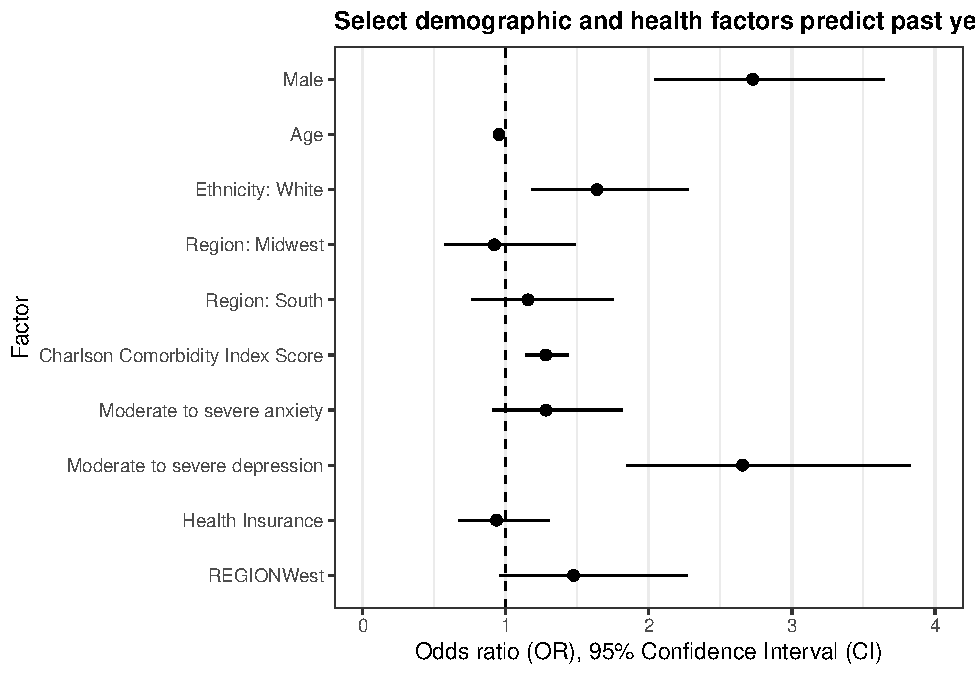
\includegraphics{PM-test_files/figure-latex/plot-1.pdf}

\begin{Shaded}
\begin{Highlighting}[]
\FunctionTok{ggsave}\NormalTok{(}\AttributeTok{filename =} \StringTok{\textquotesingle{}f1rep.pdf\textquotesingle{}}\NormalTok{, }\AttributeTok{width =} \DecValTok{9}\NormalTok{, }\AttributeTok{height =} \DecValTok{4}\NormalTok{)}
\end{Highlighting}
\end{Shaded}

\hypertarget{the-plot-for-our-replication-of-matzopoulos-morlock-morlock-lerer-lerer-2021s-multivariate-logistical-regression-resembles-the-original}{%
\subsection{The plot for our replication of Matzopoulos, Morlock,
Morlock, Lerer \& Lerer (2021)'s multivariate logistical regression
resembles the
original}\label{the-plot-for-our-replication-of-matzopoulos-morlock-morlock-lerer-lerer-2021s-multivariate-logistical-regression-resembles-the-original}}

\hypertarget{for-novel-analysis-we-elect-to}{%
\subsection{For novel analysis, we elect
to}\label{for-novel-analysis-we-elect-to}}

\end{document}
